
\documentclass[11pt, a4paper]{article}
\usepackage[font=footnotesize,labelfont=bf]{caption}
\usepackage{amsmath}
\usepackage{xcolor}
\usepackage{hyperref}
\usepackage{geometry}
 \geometry{
 a4paper,
 total={170mm,257mm},
 left=20mm,
 top=20mm,
 }
 \usepackage{graphicx}
\graphicspath{ {./Allegati/pics/} }

\title{Skyward Application \emph{- MSA department}}

\author{Andrea Stefani\thanks{andrea3.stefani@mail.polimi.it}}
\renewcommand{\labelenumi}{\alph{enumi}. } %define labels for enum
\begin{document}
\maketitle 
\vspace{2cm}
\begin{figure}[ht]
\hspace*{-0.75cm}
\begin{minipage}[b]{.45\textwidth}
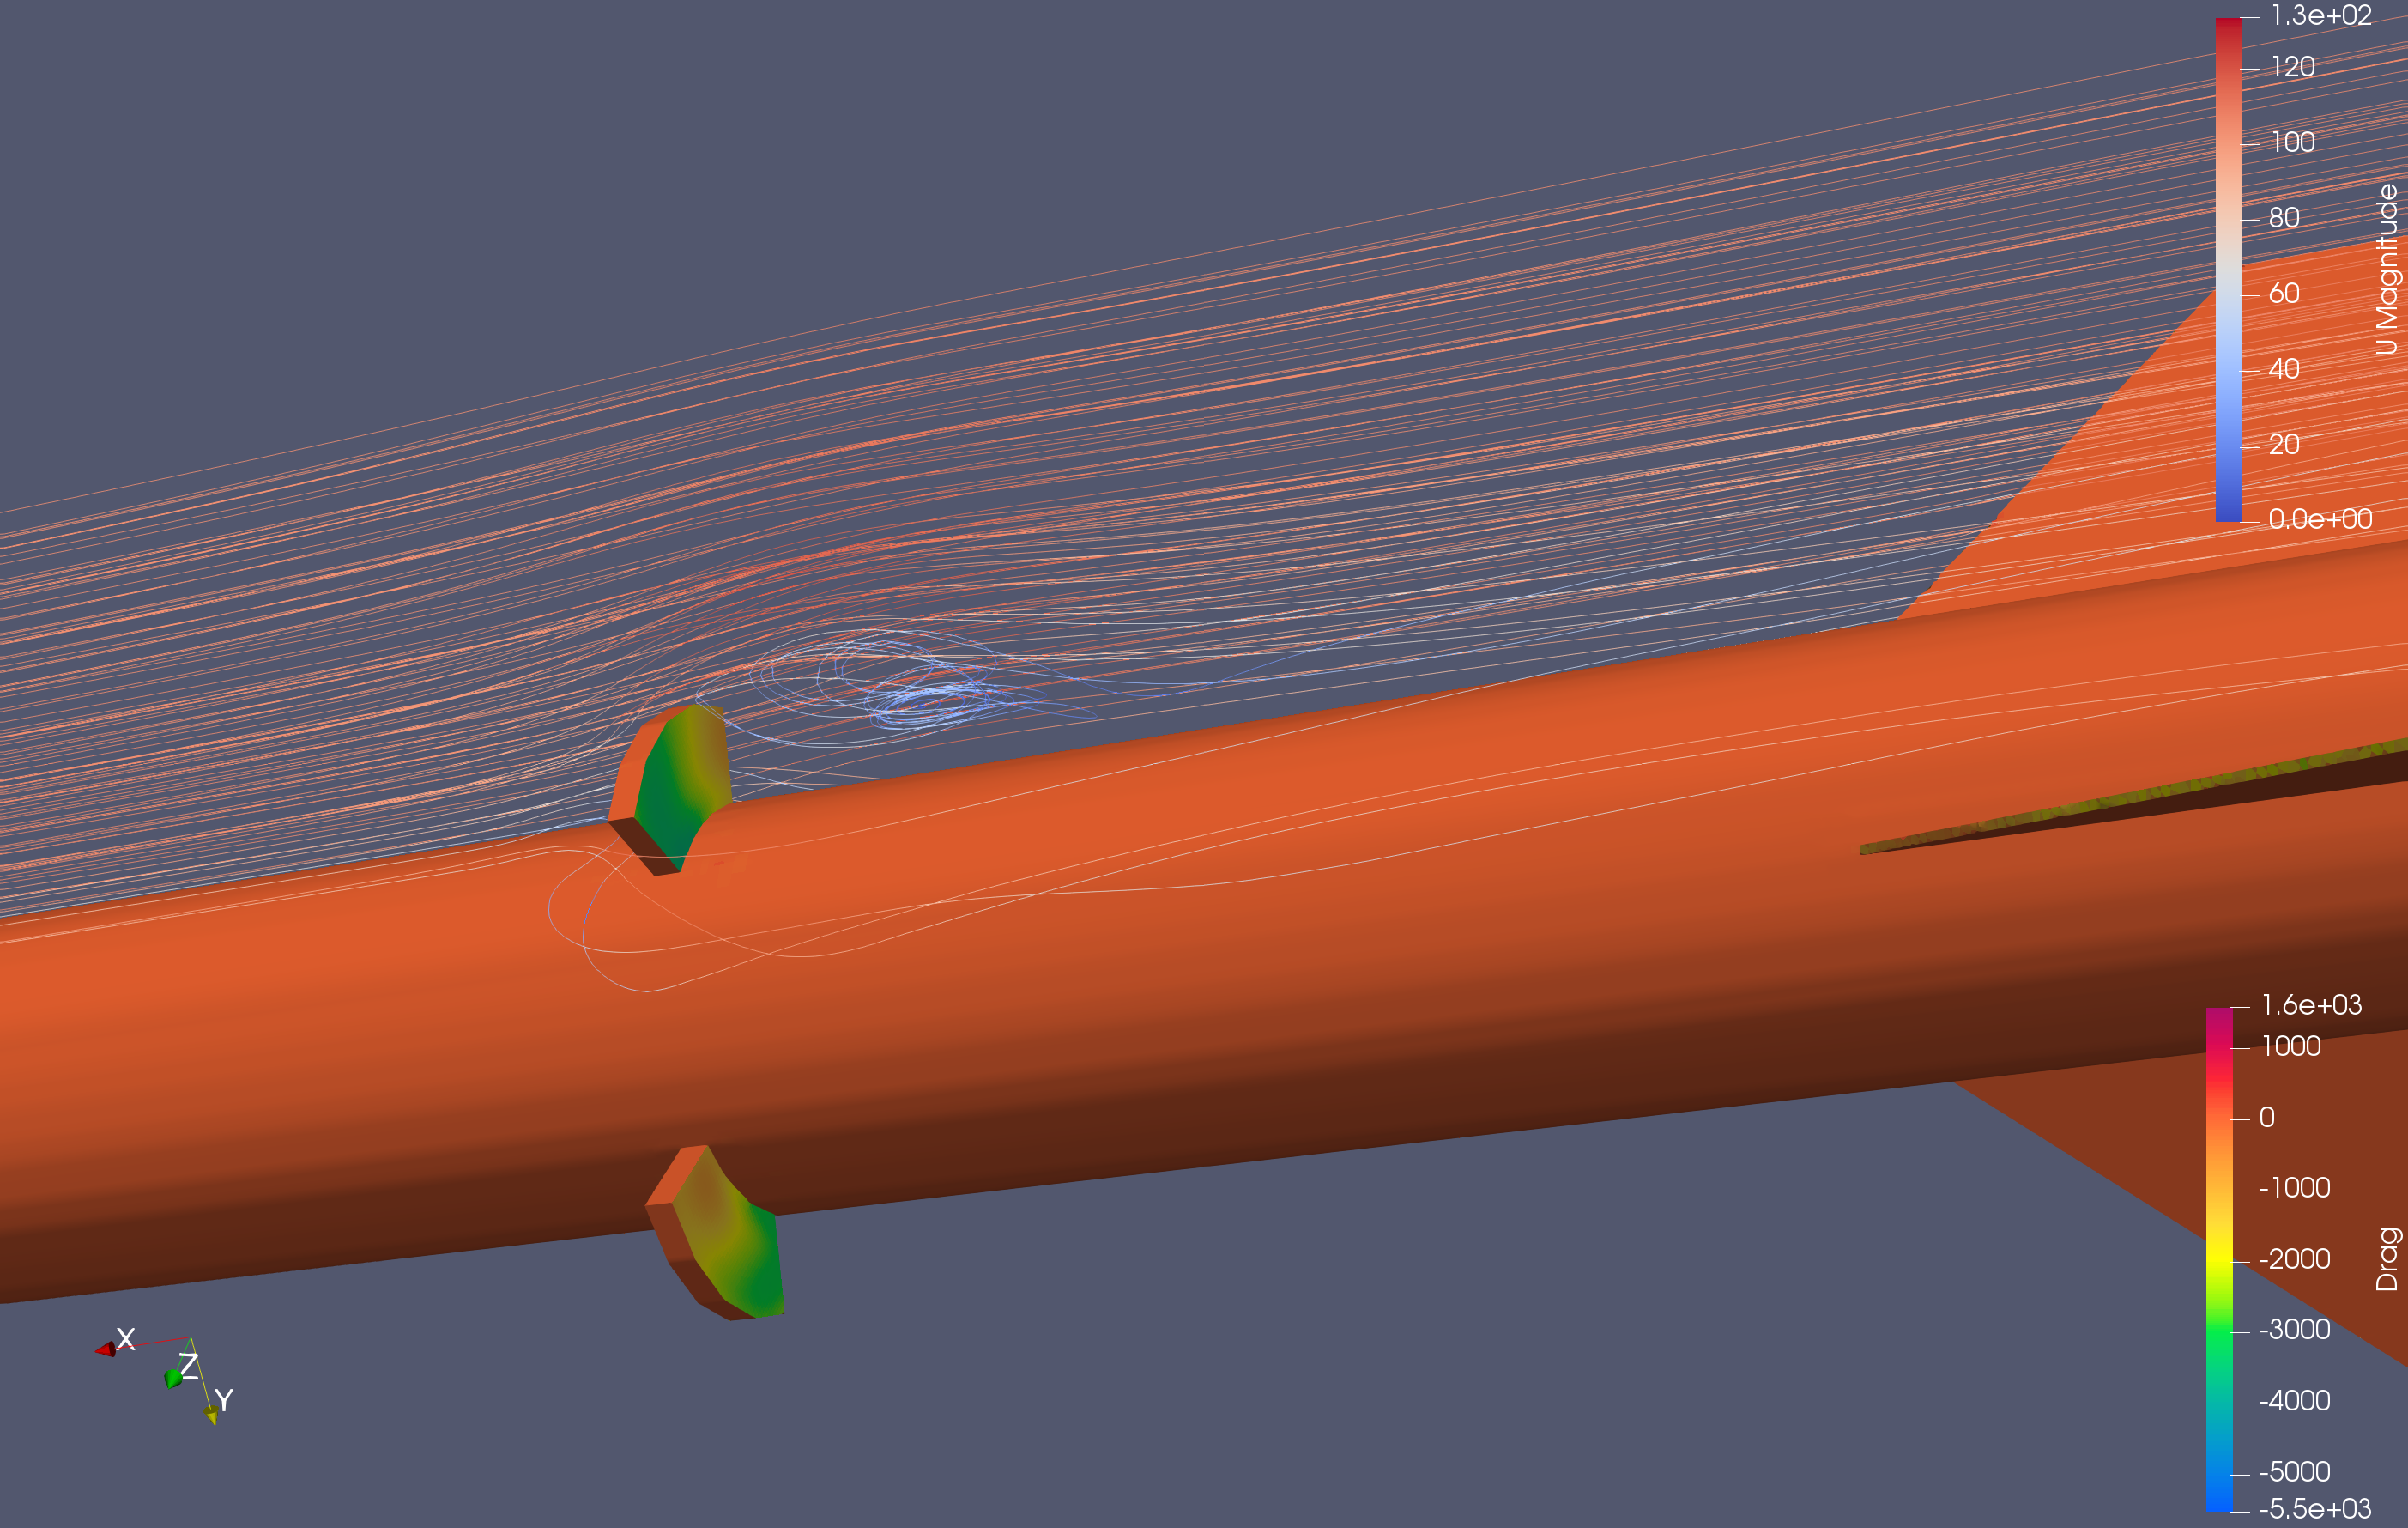
\includegraphics[scale=0.09]{brakes1}
\captionsetup{labelsep=space,justification=justified,singlelinecheck=off}
\caption{visualization of flow over airbrake and drag on the surface }
\end{minipage}
\hspace*{1.5cm}
\vspace{-0.2cm}
\begin{minipage}[b]{.45\textwidth}
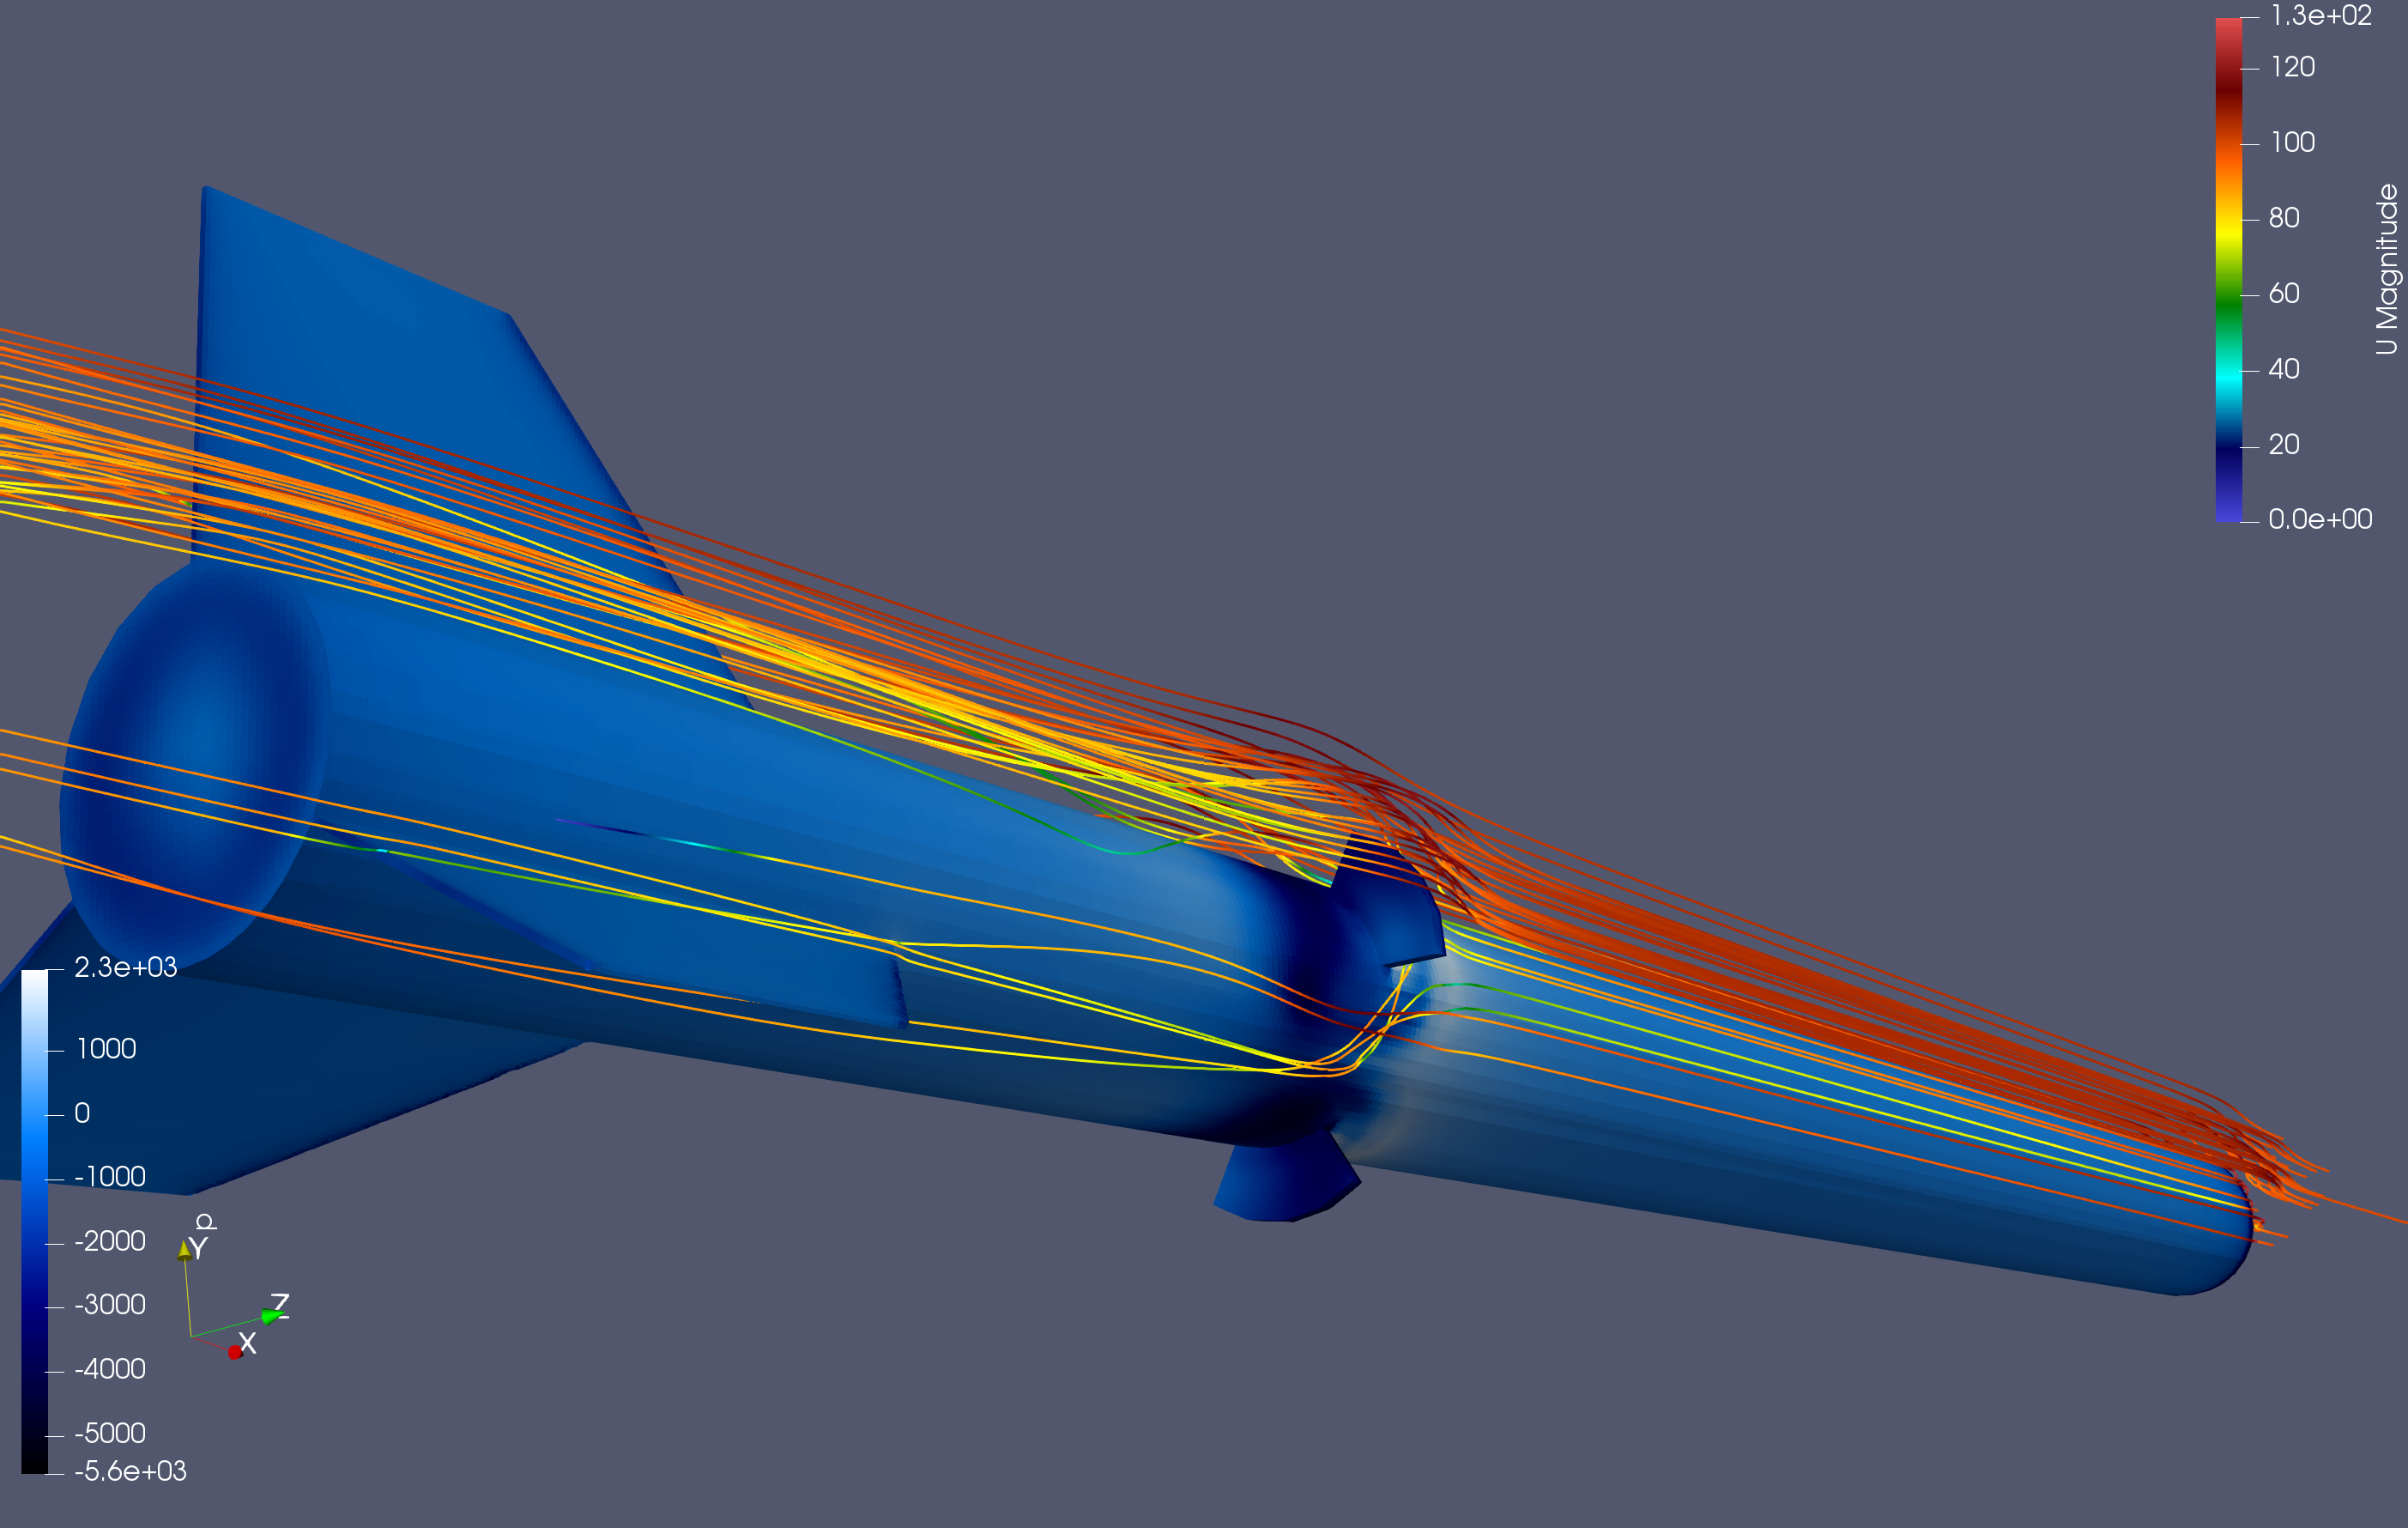
\includegraphics[scale=0.09]{brakes3}
\captionsetup{labelsep=space,justification=justified,singlelinecheck=off}
\caption{flow over airbrake and pressure over surface\newline}
\end{minipage}
\hfill
\begin{center}
\begin{minipage}[b]{.45\textwidth}
\centering
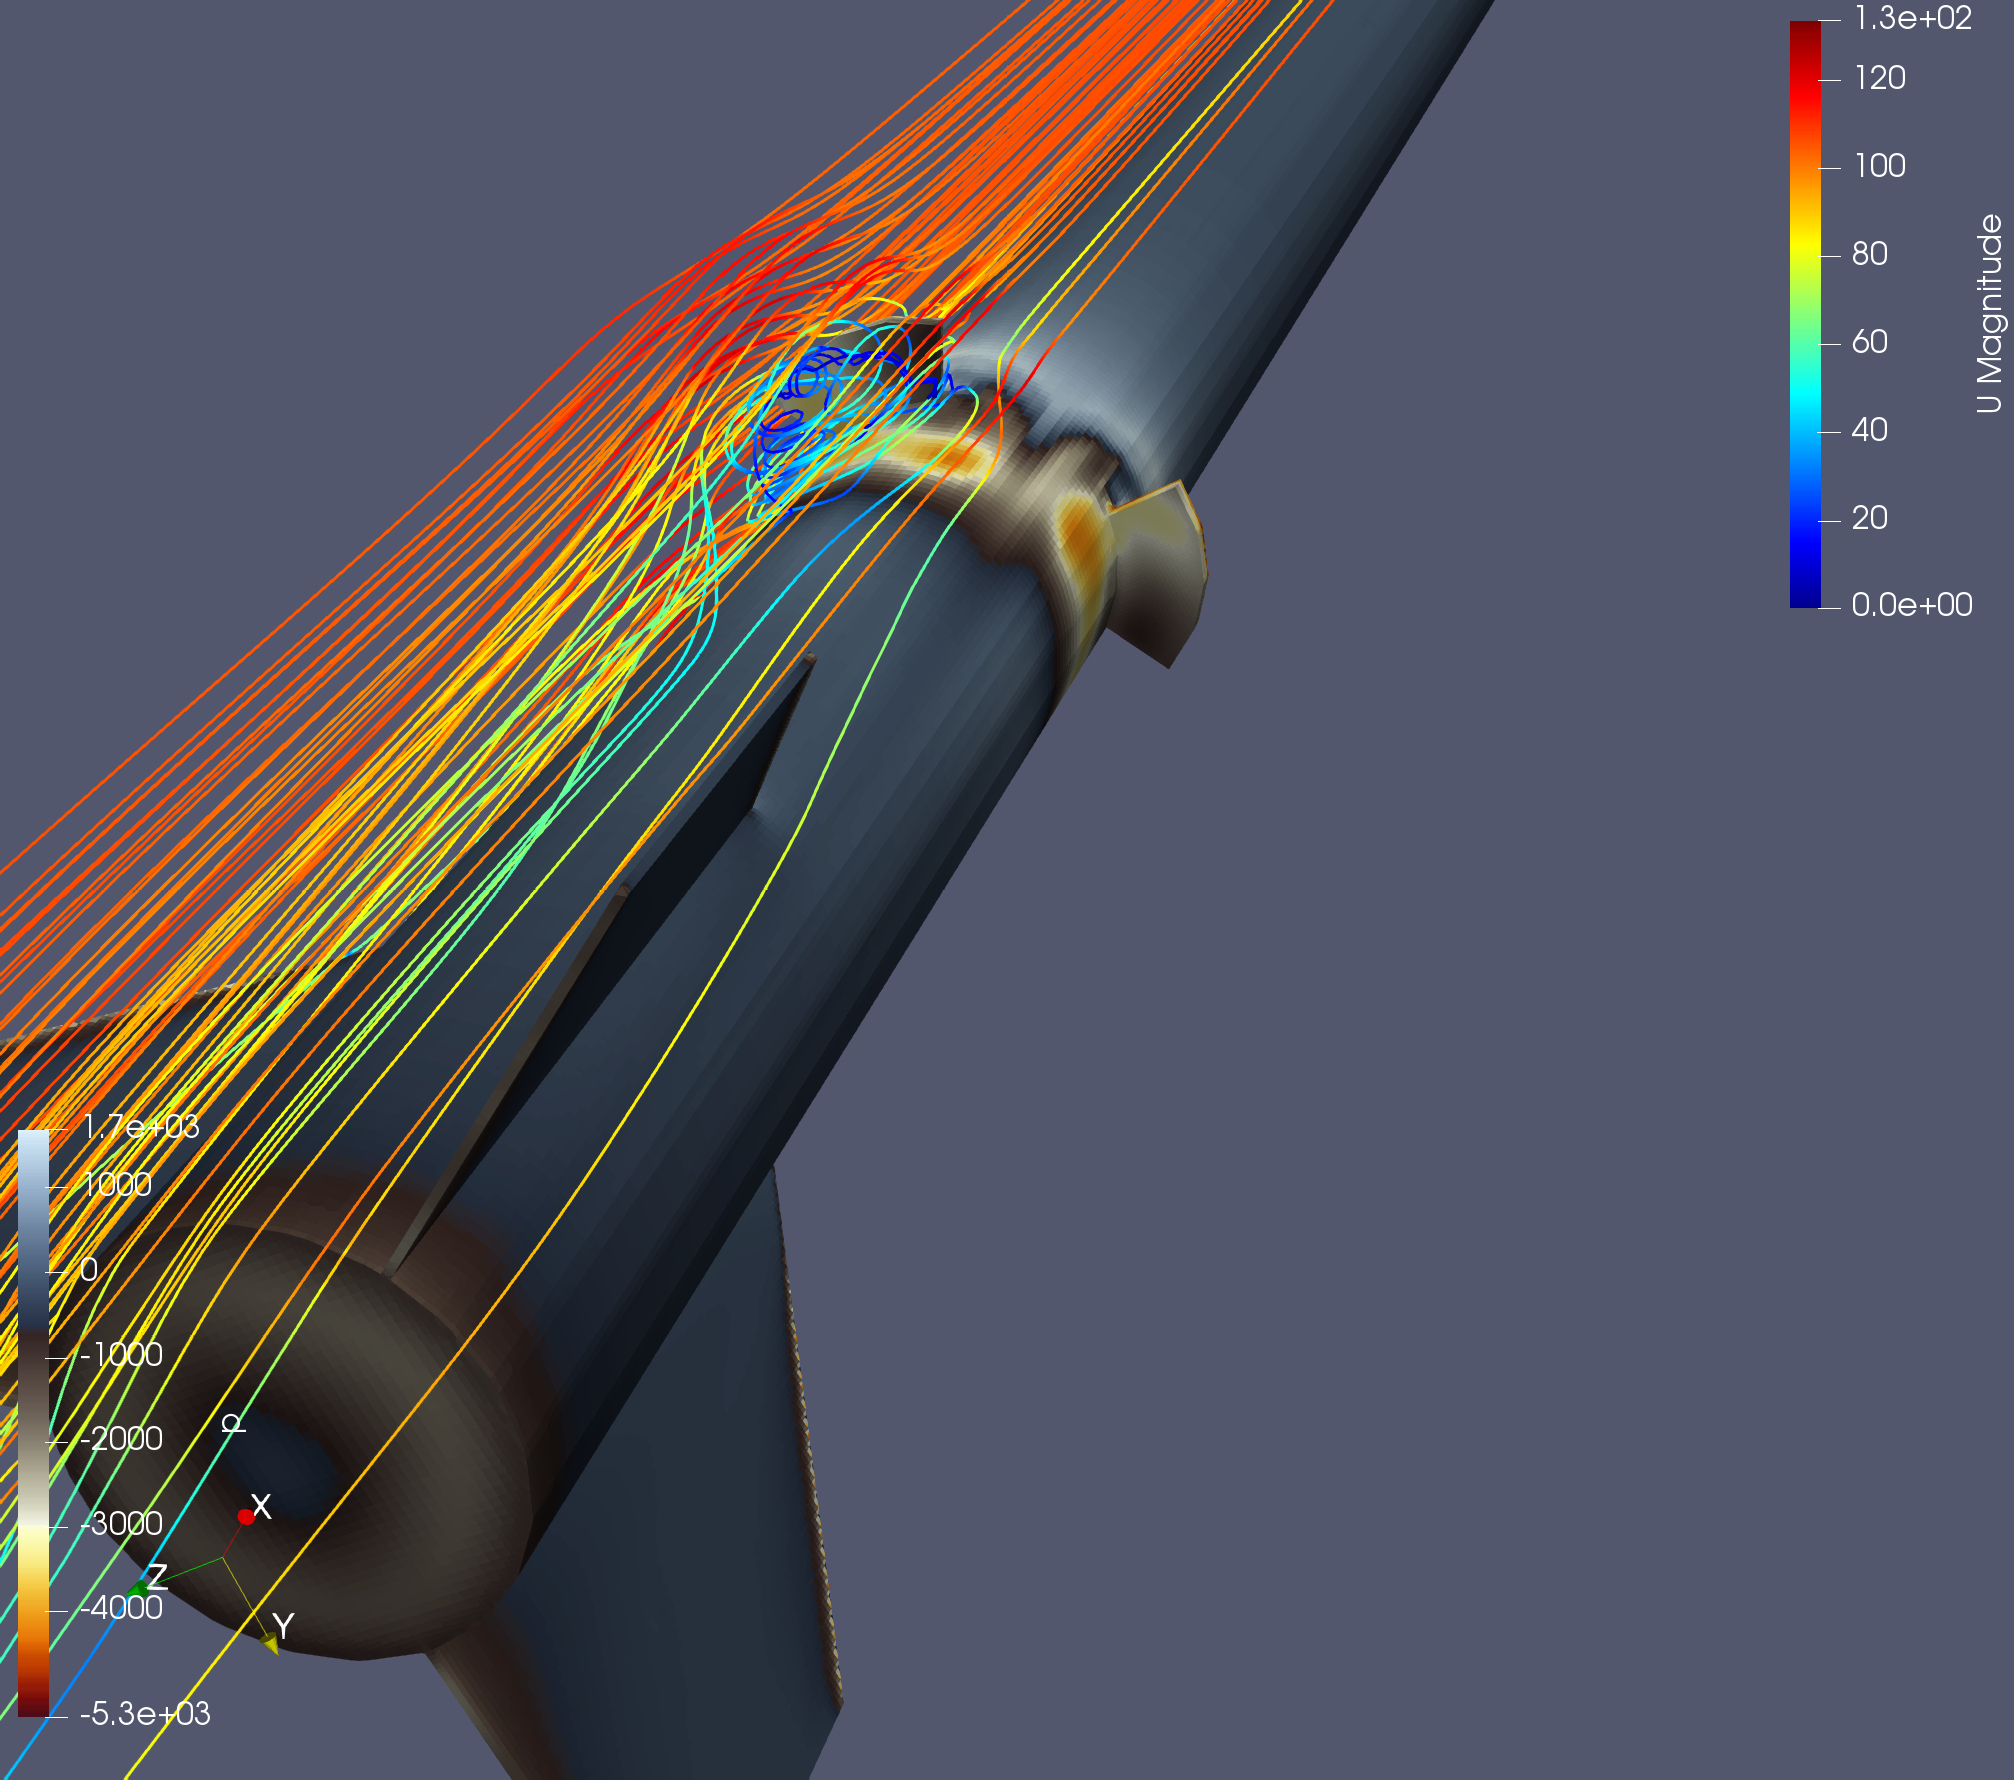
\includegraphics[scale=0.09]{brakes4}
\captionsetup{labelsep=space,justification=justified,singlelinecheck=off}
\caption{flow over airbrake and pressure over surface}
\end{minipage}
\end{center}


\end{figure}


\newpage
\vspace{10pt}
\setlength{\marginparwidth}{0pt}
\begin{enumerate}
\item Per prima cosa, come da regolamento \emph{EuroC}, è necessario consultare la lista dei motori \emph{COTS} a disposizione. Per realizzare un modello iniziale del razzo è poi necessario conoscere il \begin{math}c_d\end{math} che deve essere stimato avvalendosi di test in galleria del vento e/o simulazioni. Tramite una simulazione \emph{CFD} (rocketnobr) ho potuto stimare \begin{math}c_d=0.36\end{math}. Si può successivamente passare a realizzare un primo modello approssimato del razzo su simulink tenendo in considerazione impulso totale, massa e tempo di burnout per stimare l'apogeo. Per fare questo è inoltre fondamentale avere la curva di spinta del motore (che si può trovare su internet in formato .csv), a titolo di esempio nel mio modello ho deciso di usare la curva del motore ``M2000R'' realizzato da Aerotech e utilizzato da \emph{Skyward} sul razzo \emph{Lynx} nel 2021. Nel caso si debba scegliere da zero il motore basta consultare la lista di quelli forniti e testare ciascuna curva per verificare quale sia la migliore. Dal modello (Allegato 1) risulta un apogeo di 3500 m il che è credibile dato che in questo modello non sono presenti aerofreni. Passiamo ad analizzare i difetti del modello; prima di tutto è stata ignorata (per mancanza di tempo) la comprimibilità dell'aria, che con una velocità massima prevista che si aggira attorno a 260 m/s (0.76 Mach) non è trascurabile. A causa di questa approssimazione anche la pressione dinamica a max-q risulta abbastanza piccola da poter aprire gli aerofreni essendo lo stress, secondo un veloce calcolo (approssimando l'area di un aerofreno a 21 cm2 e lo spessore a 0.5cm), ben al di sotto persino del limite di snervamento dell'alluminio. Inoltre la simulazione in OpenFoam non considerava l'attrito radente per cui realisticamente il cd sarebbe più alto. Non potendo disporre di simulazioni CFD si potrebbe anche approssimare il valore del \begin{math}c_d\end{math} a 0.75, basandosi su dati riportati da \emph{NASA} infatti: \emph{``A typical value for the drag coefficient of a model rocket is .75, based on the cross-sectional area of the rocket''}, tuttavia questa scelta portava a risultati di apogeo meno realistici.
Per completare il modello si potrebbero per esempio considerare le condizioni atmosferiche come direzione e intensità del vento, realizzare la polare del razzo per avere stime più precise dell'attrito nelle varie condizioni, introdurre i due paracadute e utilizzare il modello anche per la stima del punto di atterraggio.
Per scegliere il motore si dovranno inoltre considerare il budget disponibile e l'accelerazione massima in relazione a quella sopportabile dal payload.
\item Per il funzionamento degli \emph{aerofreni} è fondamentale una discreta velocità del \emph{vento relativo}, in modo da generare sufficiente attrito da rallentare il razzo, tuttavia, aprirli troppo presto risulterebbe in una sollecitazione meccanica troppo elevata che ci costringerebbe a realizzare aerofreni più resistenti e quindi pesanti. Nonostante i risultati della simulazione precedente (per quanto detto su max-q) credo che aprire gli aerofreni troppo presto rischierebbe di romperli o quanto meno superare il limite di snervamento. Inoltre, aprendo gli aerofreni più tardi possibile \emph{si riduce l'incertezza} sull'apogeo calcolato, dato che questo dipenderà da meno fattori incogniti. D'altra parte, aprirli troppo tardi gli da meno tempo per frenare a sufficienza. Per questi motivi aprirei gli aerofreni sicuramente dopo lo spegnimento del motore e superato il punto di \emph{max-q} a cui si massimizza la formula: \begin{math} 1/2\rho v^2\end{math} e con essa le forze aerodinamiche, lasciando il compito di decidere il momento preciso al modello descritto al punto e).
\item L'apertura degli aerofreni crea (come evidenziato da Allegato2 e figure 1 2 3) una separazione del flusso, questo causa una perdita di portanza nell'ultima parte del razzo evidenziata nelle immagini da aree di bassa pressione dopo gli erofreni. Tuttavia, la portanza è per la maggior parte fornita dalle alette mente quella fornita dalla struttura del razzo è trascurabile, per cui basterebbe evitare che la separazione del flusso colpisca le alette. Questo può essere fatto ponendo le alette sfalsate rispetto agli aerofreni e/o dimensionandoli in modo che la separazione non coinvolga le alette. Dalla simulazione in OpenFoam (rocket2) si nota come la dimensione e distanza degli aerofreni dalle alette sia sufficiente a evitare che le zone di bassa pressione raggiungano le alette.
\item Andrebbero considerati anche gli effetti dinamici sul flusso a valle degli aerofreni, per questo sarebbe più utile una simulazione LES che modelli anche le turbolenze. Se queste infatti impattano sulle alette potrebbero avere comunque effetti sul loro funzionamento e sull'assetto del razzo. Tuttavia, analizzando il flusso generato dalla simulazione OpenFoam (rocket2) posso ragionevolmente, seppure con le solite riserve riguardanti la comprimibilità, ipotizzare che porre gli aerofreni sfalsati rispetto alle alette eviti o quanto meno limiti gli effetti indesiderati delle turbolenze.
\item  Utilizzerei per controllarne l'apertura un modello che stimi l'apogeo tenendo conto di velocità e quota, calcolate tramite integrazioni successive dell'accelerazione, e Forze applicate al razzo (attrito, gravità). Le misure barometriche possono essere combinate con questo calcolo per rendere la misura più accurata. Si può poi implementare un controllo automatico che apra gli aerofreni imponendo le condizioni \newline \begin{math} 1/2\rho v^2 < p_{max}\end{math} \newline dove \begin{math}p_{max}  \end{math} è la massima pressione aerodinamica sopportabile dagli aerofreni e \newline\begin{math} h_{est} > 3000\end{math} \newline ovvero l'apogeo atteso è minore di quello voluto di 3000m. In queste condizioni si aprono gli aerofreni. Nell'esempio fornito (Allegato2) l'apogeo viene stimato semplificando il problema a una sola dimensione, la quota. L'apogeo non viene in realtà stimato ma si procede applicando la formula oraria \begin{math}h=h_0 + v_0t + 1/2at^2+ 1/6jt^3 \end{math} dove j è lo strappo, ovvero la derivata dell'accelerazione. Si utilizza questa formula calcolando il suo valore per 10 istanti successivi e si prende poi il maggiore di essi confrontandolo con 3000m. 



\end{enumerate}
Note:
\begin{itemize}
	
	\item La velocità del flusso in entrambe le simulazioni OpenFoam è 100m/s, l'algoritmo utilizzato è simpleFoam.
	\item Tutti i risultati a cui si fa riferimento sono consultabili dai modelli nella cartella \color{blue}\href{file:./Allegati/.}{/Allegati} \color{black} e dalle foto nella cartella \color{blue}\href{file:./Allegati/pics/.}{/Allegati/pics}. \color{black}Le cartelle complete delle simulazioni si possono trovare su github \color{blue}\href{https://github.com/andrea-st1701/CFD_rocket}{github} \color{black}
\end{itemize}
Made with \LaTeX


\end{document}